% !TEX root = main.tex
%%%%%%%%%%%%%%%%%%%%%%%%%%%%%%%%%%%%%%%%
%%%%%%%%%%%%%%%%%%%%%%%%%%%%%%%%%%%%%%%%
\section{\approach} \label{sec:t5}
%%%%%%%%%%%%%%%%%%%%%%%%%%%%%%%%%%%%%%%%
%%%%%%%%%%%%%%%%%%%%%%%%%%%%%%%%%%%%%%%%

We start by providing an introduction to the T5 model we use (\secref{sub:t5}). Then, we describe how we built the datasets used for the different training phases we dealt with (\secref{sub:datasets}).  \secref{sec:training} will then explain how we used these datasets to run the actual training process.


\subsection{Text-to-Text-Transfer-Transformer (T5)}
\label{sub:t5}
T5 has been introduced by Raffel \etal \cite{raffel2019exploring} as a Transformer \cite{vaswani2017attention} model to support multitask learning in the domain of NLP (Natural Language Processing). The idea behind the T5 model is to reframe NLP tasks in a unified text-to-text format in which the input and output of the model are text strings. This implies that a single model can be trained to translate across languages (\eg from English to Spanish) and to autocomplete sentences. The training of T5 includes two phases. The first is the \textit{pre-training}, in which the model is trained with a self-supervised objective to acquire general knowledge about the language(s) of interest. In our example, this may mean providing as input to the model English sentences having a subset of their words masked and asking the model to generate as output the masked words. Being self-supervised (\ie the training instances can be automatically generated by masking random words) the pre-training can usually be performed on large-scale datasets. Once pre-trained, T5 can be fine-tuned to support specific tasks with supervised training objectives. This means, for example, providing it with pairs of sentences $<$\emph{english}, \emph{spanish}$>$.

In our work, we rely on the same T5 architecture (\ie T5$_{small}$) that has been exploit by Mastropaolo \etal \cite{mastropaolo2022using} in LANCE. T5\textsubscript{\textit{small}} is characterized by six blocks for encoders and decoders. The feed-forward networks in each block consist of a dense layer with an output dimensionality ($d_{ff}$) of 2,048. The \textit{key} and \textit{value} matrices of all attention mechanisms have an inner dimensionality ($d_{kv}$) of 64, and all attention mechanisms have eight heads. All the other sub-layers and embeddings have a dimensionality ($d_{model}$) of 512. The code implementing T5 is available in our replication package \cite{replication}.


\subsection{Datasets Needed for Training, Validation, and Testing}
\label{sub:datasets}

We start by describing the dataset used for pre-training T5 (\secref{sub:pretraining}). Then, we detail the several fine-tuning datasets we built (featuring training, validation, and test set). The first, aimed at replicating LANCE \cite{mastropaolo2022using}, teaches T5 how to inject a single log statement in a Java method  (\secref{sec:single-log-dataset}). The second fine-tuning dataset also focuses on the problem of injecting a single log statement, but this time exploits IR to provide T5 with concrete examples of log messages that might be relevant for the prediction at hand (\secref{sec:single-log-plus-IR}). This allows to directly compare LANCE with \approach in the task of single log statement generation. The third fine-tuning dataset trains \approach for the task of multi-log statements prediction, \ie the ability to inject from 1 to $n$ log statements in a given method (\secref{sec:multi-log-dataset}). Also this fine-tuning dataset exploits IR to boost the prediction accuracy. Finally, we show how we built a fine-tuning dataset to tech T5 how to discriminate between methods needing and not needing log statements (\secref{sec:predicting-dataset}). The datasets are summarized in \tabref{tab:ds-summary-1} and \tabref{tab:ds-summary-2}.



All datasets have been built starting from the same set of GitHub repositories that we selected using the GHS (GitHub Search) tool by Dabi\'c \etal \cite{dabic2021sampling}. GHS allows to query GitHub for projects meeting specific criteria. We used the same selection criteria by Mastropaolo \etal \cite{mastropaolo2022using}, selecting all public non-forked \java projects having at least 500 commits, 10 contributors, and 10 stars. These selection criteria aim at excluding personal/toy projects and reduce the chance of collecting duplicated code (non-forked repositories). We cloned the latest snapshot of the 6,352 projects returned by GHS. We scanned all cloned repositories to assess whether they featured a \texttt{POM} (Project Object Model) or a \texttt{build.gradle} file. Both these files allow to declare external dependencies towards libraries, the former using Maven, the latter Gradle. Such a check was performed since, as a subsequent step, we verify whether projects had a dependency towards Apache Log4j \cite{log4j} (\ie a well-known Java logging library) or SLF4J (Simple Logging Facade for Java) \cite{slf4j} (\ie an abstraction for Java logging frameworks similar to Log4j). Indeed, to train a T5 for the task of injecting complete log statement(s) in Java methods, we needed examples of methods featuring log statements. The usage of popular logging Java libraries was thus a prerequisite for the project's selection.

We found 3,865 projects having either a \texttt{POM} or a \texttt{build.gradle} file and 2,978 of them featured a dependency towards the two targeted logging libraries. The overall projects' selection is very similar to the one by Mastropaolo \etal \cite{mastropaolo2022using}, with the main differences being the additional mining of projects: (i) using Gradle as build system (in \cite{mastropaolo2022using} only Maven was considered); and (ii) having a dependency towards SLF4J (in \cite{mastropaolo2022using} only Log4j was considered as logging library). These choices help in increase the size and variety of both the training and the testing datasets, making the prediction more challenging. 

We then used srcML \cite{srcml} to perform a lightweight parsing of the selected projects. First, we extracted all \java methods they feature. Then, we identified the log statements within each method (if any) and removed all methods featuring log statements exploiting custom log levels (\ie log levels that do not belong to any of the two libraries we consider in our study but that have been defined within a specific project). The valid log levels we considered are: \texttt{FATAL}, \texttt{ERROR}, \texttt{WARN}, \texttt{DEBUG}, \texttt{INFO}, and \texttt{TRACE}. At this point we were left with two sets of methods: those not having any log statement and those having at least one log statement using one of the ``valid'' log levels.

We run \emph{javalang} \cite{javalang} on the remaining methods to tokenize them and excluded all those having $\#tokens < 10$ or $\#tokens \geq 512$. The upper-bound filtering has been done in previous works \cite{ADD_CITATIONS_FROM_OTHER_GROUPS,mastropaolo2021empirical,tufano2021automating,ciniselli2021empirical} to limit the computational expenses of training DL-based models. The lower-bound of 10 tokens aims at removing empty methods. We also filtered out all the methods containing non-ASCII characters in an attempt to exclude at least some of the methods featuring log messages not written in English. 


Finally, to avoid any possible overlap between the training, evaluation, and test datasets we are going to create from the collected set of methods, we removed all exact duplicates, obtaining the final set of 12,917,300 \java methods, of which 244,588 contain at least one log statement. 

\begin{table*}[h]
	\centering
	\caption{Number of methods in the datasets used in our study}
		\label{tab:ds-summary-1}
	\begin{tabular}{ccccccccc}
		\toprule
		\multirow{2}{*}{\textit{\textbf{Dataset}}} & \multicolumn{2}{c}{\textbf{train}} & \textbf{} & \textbf{eval} & \textbf{} & \textbf{test}  \\ \cline{2-3} \cline{5-5} \cline{7-7} 
		& \textbf{w/ log} & \textbf{w/o log} & \textbf{} & \textbf{w/ log} & \textbf{} & \textbf{w/ log} \\ \midrule
		\textit{Pre-training}              & -               &      12,671,475  &           & -               &           &  -               \\
		\textit{Fine-tuning: Single Log Generation}               & 229,703         & -                &           & 28,763          &           & 28,698          \\
		\textit{Fine-tuning: Single Log Generation with IR}               & 229,703         & -                &           & 28,763          &           & 28,698          \\
		\textit{Fine-tuning: Multi-log Injection with IR}               & 192,773         & -                &           & 24,092         &           & 24,088          \\
		\bottomrule
	\end{tabular}
\end{table*}

\subsubsection{Pre-Training Dataset}
\label{sub:pretraining}
Since the goal of pre-training is to provide T5 with general knowledge about the language of interest (\ie Java), we used for pre-training all methods not featuring a log statement (the latter will be used for the fine-tuning datasets). For the pre-training we adopted a classic \emph{masked language model} task, which consists in randomly masking 15\% of the tokens composing a training instance (\ie a Java method in our case) asking the model to predict them. \figref{fig:pre-training} depicts a pre-training instance from our dataset.


\begin{figure}[h!]
	\label{fig:ir-example}
	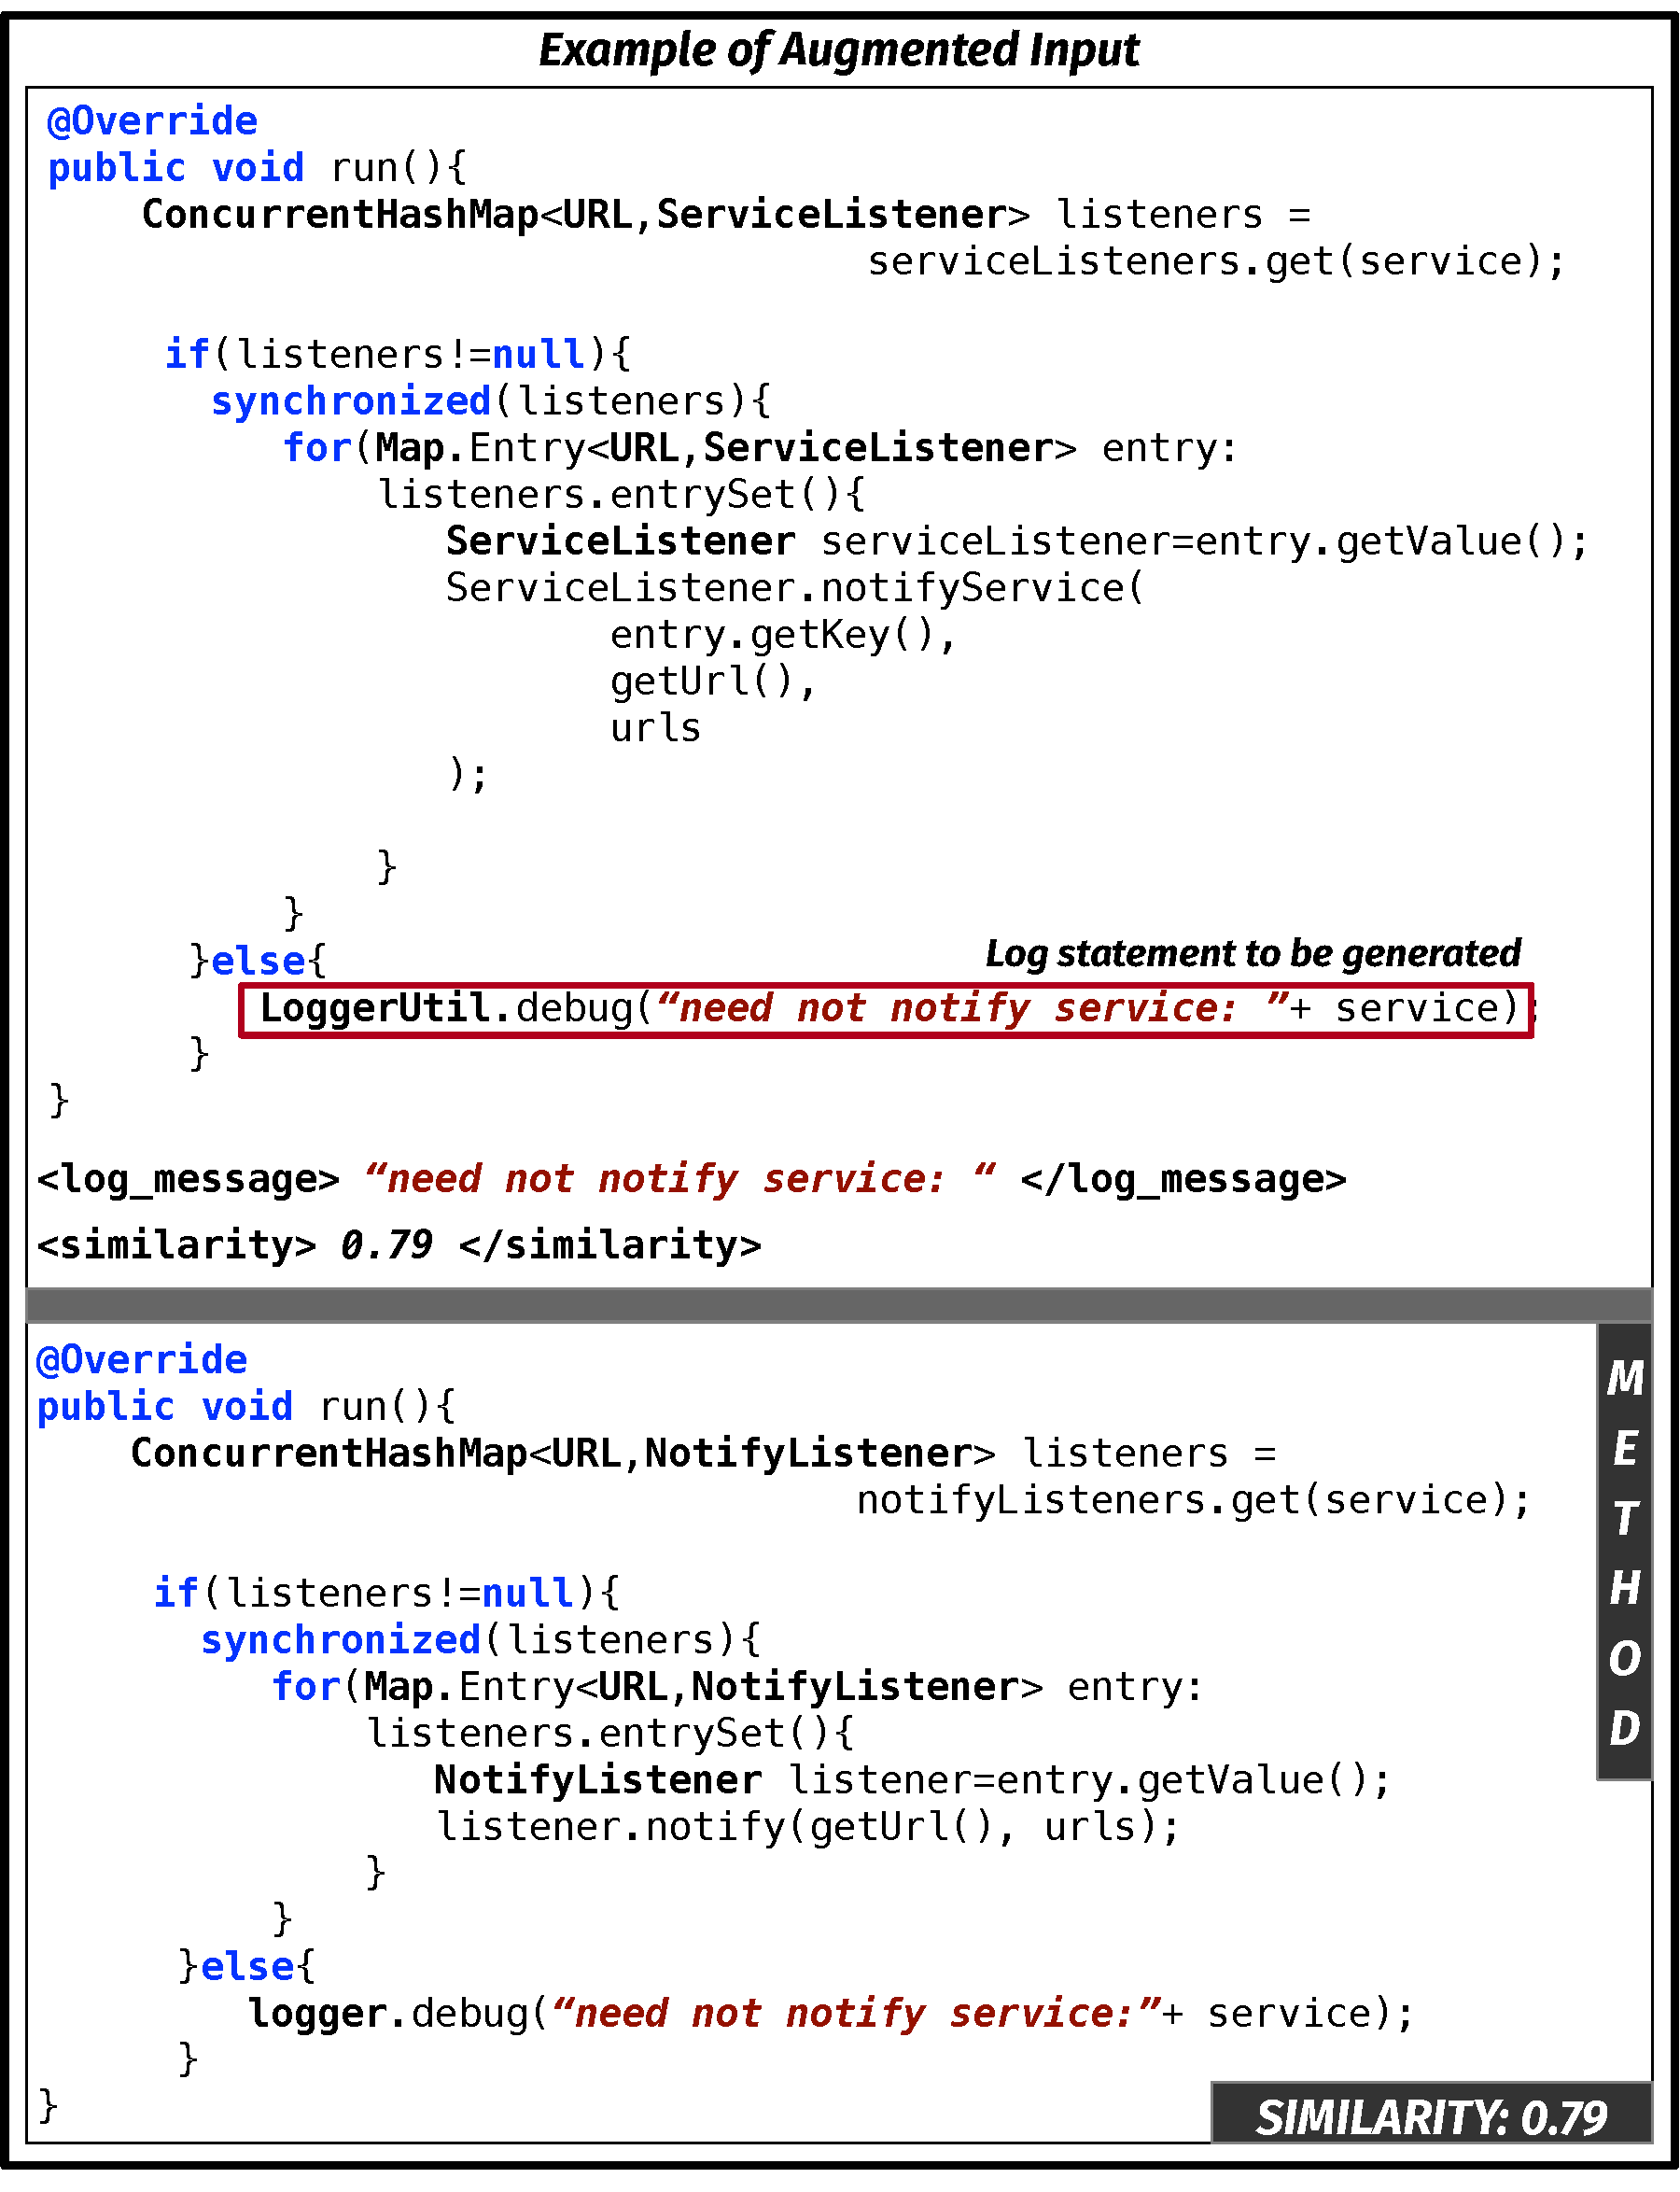
\includegraphics[width=\columnwidth]{img/ir-example.pdf}
	\caption{Example of augmented input featured by log messages retrieved from the ($k=3$) most similar coding context.}
\end{figure}

\begin{figure}[h!]
	\label{fig:pre-training}
	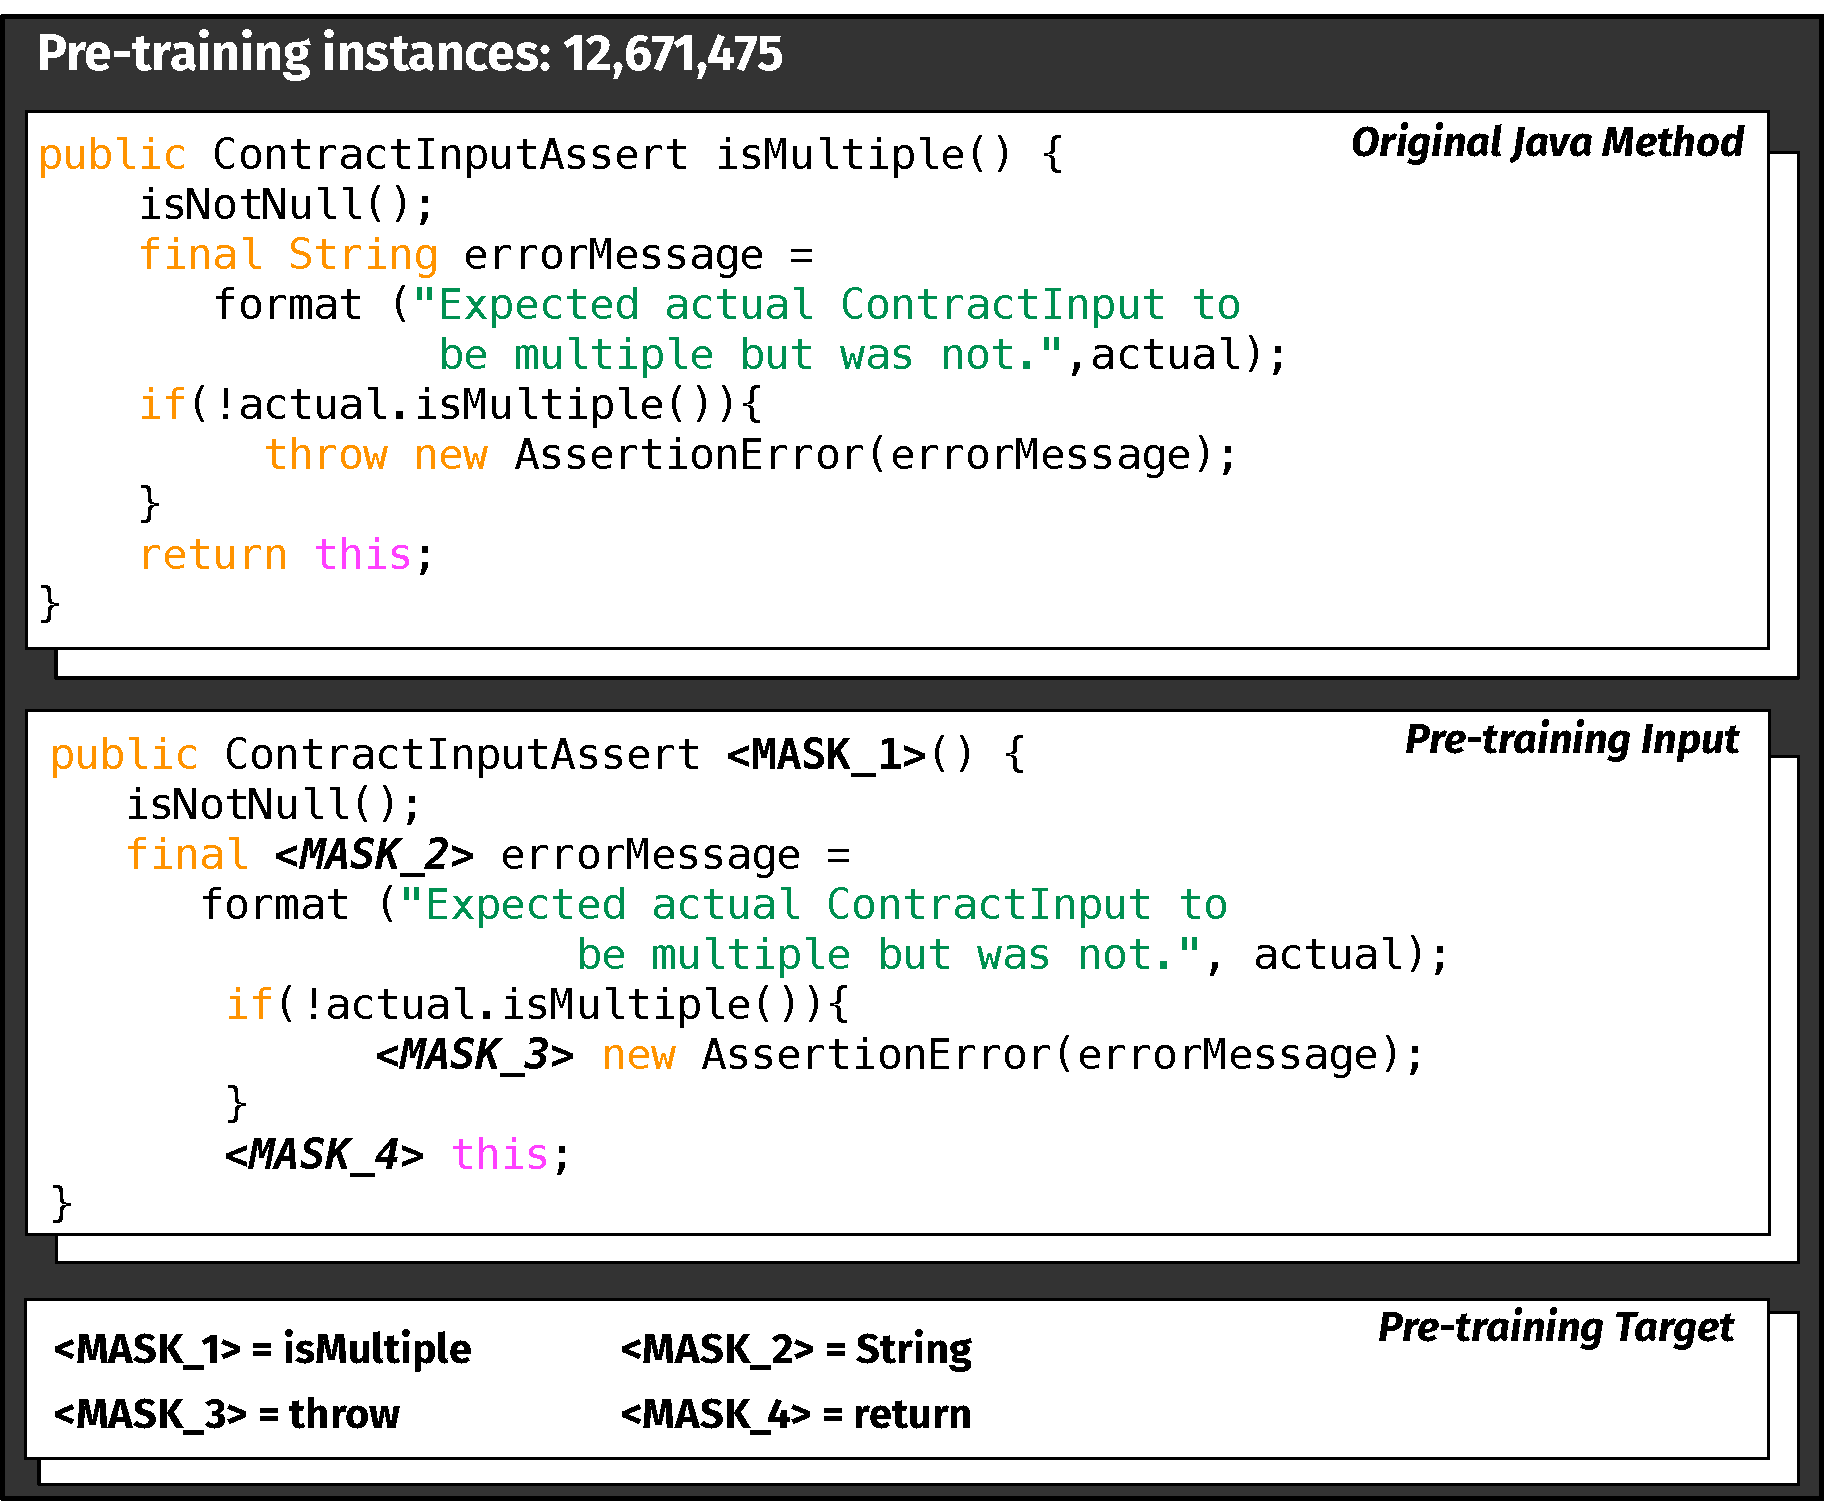
\includegraphics[width=\columnwidth]{img/pre-training.pdf}
		\caption{Example of Pre-training instance}
\end{figure}



\subsubsection{Fine-tuning Dataset: Single Log Generation} \label{sec:single-log-dataset}
We build a fine-tuning aimed at replicating what has been done in the training of LANCE by Mastropaolo \etal \cite{mastropaolo2022using}. We process each method $M$ having $n \geq 1$ log statements by removing from it one log statement (\ie leaving it with $n-1$ log statements). This allows to create a training pair $\langle M_s, M_t \rangle$ with $M_s$ representing the input provided to the model (\ie $M$ with one removed log statement) and  $M_t$ being the expected output (\ie $M$ in its original form, with all its log statements). This is the dataset used to train LANCE \cite{mastropaolo2022using} and it allows to train a model able, given a Java method as input, to inject in it one new log statement. 

For methods having $n > 1$ (\ie more than one log statement), we created $n$ pairs $\langle M_s, M_t \rangle$, each of them having one of the $n$ log statements removed (\ie different $M_s$). To ensure that after the log statement removal our instances still featured valid Java methods, we parsed each $M_s$ using JavaParser \cite{javaparser} and removed all pairs including an invalid $M_s$. 

We split the remaining pairs into training (80\%), validation (10\%) and test (10\%) set as reported in \tabref{tab:ds-summary-1}. Training and testing a T5 model on this dataset basically means performing a differentiated replication of LANCE on a much larger (+\textcolor{red}{XX\%} of instances) and more variegate (multiple logging libraries) dataset.

\subsubsection{Fine-tuning Dataset: Single Log Generation with IR} \label{sec:single-log-plus-IR}

In \approach, we want to combine DL and IR with the goal of boosting performance especially when it comes to the generation of meaningful log messages, being one of the weaknesses of LANCE. The main idea is to augment the input provided to the model (\ie $M_{s}$) with log messages belonging methods similar to $M_{s}$ which are featured in the fine-tuning training set. For each of the 244,588 $\langle M_s, M_t \rangle$ pairs in the fine-tuning dataset described in \secref{sec:single-log-dataset} (this includes training, validation, and test), we identify the $k$ most similar pairs in the training set. The similarity between two pairs is based on the similarity of their $M_s$ (\ie the method in which the log statement must be created) and it is computed using the Jaccard similarity \cite{hancock2004jaccard} index, based on the percentage of code tokens shared across the two methods. We then use these $k$ similar methods to extract from them example of log messages used in coding contexts which are similar to the $M_s$ at hand. Two clarifications are important here. First, independently if a given pair is in the training, validation, or test set, we extract its $k$ most similar pairs only from the training set. This is needed since, while predicting the log statement to inject, the training set must be the only knowledge available to the model (\ie the test set must be composed of previously unseen instances). Second, when computing the Jaccard similarity, we remove from the compared methods all log statements, since we want to identify similar ``coding contexts'' that may require similar log statements. We created three different fine-tuning datasets using different values of $k=\{1,3,5\}$ (thus, a higher/lower number of exemplar log messages provided as input to the model).




\figref{fig:ir-example} shows an example of training instance for this fine-tuning dataset. The method on top represents the $M_{s}$ \java method in which a log statement must be injected (\ie the one highlighted in red). The method is enriched with the exemplar log messages that have been found in the $k=3$ most similar methods shown in the bottom. Besides the log messages, we also provide T5 with the Jaccard similarity between the $M_{s}$ at hand (top of the figure in this case) and the method of the training set from which each log message has been extracted. This is just meant to represent an additional hint for T5 in terms of which exemplar message comes from the most similar coding context.

Note that the instances in this dataset are exactly the same of the one previously described to replicate LANCE (see \tabref{tab:ds-summary-1}). This allows a direct comparison in terms of performance which will provide information about the gain, if any, provided by the integration of the IR technique in the loop.

\subsubsection{Fine-tuning Dataset: Multi-log Injection with IR} \label{sec:multi-log-dataset}

The second limitation of LANCE \cite{mastropaolo2022using} we aim at addressing is the assumption that a Java method provided as input always require one new log statement to be injected. Also for this dataset, \approach exploits a combination of DL and IR, thus we follow a process similar to the one described in \secref{sec:single-log-plus-IR}, with the main difference being the number of log statements we ask the model to generate. In particular, given a method $M$ featuring $n$ log statements, we randomly select $y$ log statements to remove from it, with $1 \leq y \leq n$. This means that in this case we create pairs $\langle M_s, M_t \rangle$ in which $M_s$ lacks a ``random'' number of log statements that must be generated by the model to obtain the target method $M_t$. This makes the prediction task substantially more challenging as compared to the single-log injection scenario experimented in LANCE. Also in this case we parsed each $M_s$ using JavaParser \cite{javaparser} and removed all pairs including an invalid $M_s$. The remaining part of the process (\ie identifying the $k$ most similar pairs to inject examples of log messages) is exactly the same as the one described in \secref{sec:single-log-plus-IR}. \tabref{tab:ds-summary-1} shows the distribution of instances among the training, evaluation, and test set for this dataset as well.

%%%STOPPED HERE

\subsubsection{Fine-tuning Dataset: Deciding Whether Log Statements are Needed} \label{sec:predicting-dataset}

To build the dataset needed for predicting whether or not log statements are needed in a \java method, we use the same set of instances featuring the dataset built for the multi-log injection model. To this extent, we start from the original set of 244,588 \java methods having at least one log statement, then for each method, we chose an arbitrary number $k$ from 0 to $n$, where $n$ is the number of log statements in the method. Then, we randomly selected $k$ log statements out of the
method's $n$ logs. When $k$ is equal to 0 it means that no log statements have been removed and, thus, the input sequence and the target sequence are equal (\ie, the original \java method). After the log statements removal, we ensured that the input sequences still represented a valid \java code by using JavaParser \cite{javaparser} to parse the methods. All those instances throwing parsing exceptions have been removed from the datasets. 
Finally, for each instance, we replaced the target sequence with a binary choice either \texttt{Need} or \texttt{No need}. Instances labeled as \texttt{No need} correspond to the entries for which no log statements have been removed (\ie $k=0$) thus, need no further logs. On the other hand, the entries labeled as \texttt{Need} are those missing at least one log statement. It is possible that two methods differ only because they contain a different log statements, if said statements are removed then the methods could be considered equal. Thus, input sequences pointing to the same target sequences (\ie \texttt{Need}), have been removed to avoid duplicated entries in the dataset obtaining a training and a validation set feature by 190,974 instances and 23,725 respectively.

As for the test set, since it is not possible to ensure it represents the real distribution of Java methods that either need or do not need log statements, we decided to test the model's performance on three different test sets. Each test set contains a different distribution in terms of Java methods that need the injection of further logs or not. To this extent, we create three distributions:  (i) 50-50 (50\% of the instances require at least one additional log statement, the other 50\% do not), (ii) 75-25 (75\% of the methods want at least one additional log statement while the remaining 25\% do not) and, (iii) 25-75 (25\% of the instances need the injection of at least one log statements, while the other 75\% need none).
\tabref{tab:ds-summary-2} reports the number of instances contained in the above-mentioned datasets.

\begin{table*}[h!]
	\centering
	\caption{Num. of methods in the datasets used to predict the need for logs}
	\begin{tabular}{rcccccccc}
		\hline
		\multirow{2}{*}{\textit{\textbf{Dataset}}} & \multicolumn{2}{c}{\textbf{train}} & \textbf{} & \multicolumn{2}{c}{\textbf{eval}}  & \textbf{} & \multicolumn{2}{c}{\textbf{test}}  \\ \cline{2-3} \cline{5-6} \cline{8-9} 
		& \textbf{Need} & \textbf{No need}   & \textbf{} & \textbf{Need} & \textbf{No need}   & \textbf{} & \textbf{Need} & \textbf{No need}   \\ \hline
		\textit{Need4Log fine-tuning dataset (50-50)}         & 98,848        & 92,126             &           & 12,257        & 11,468             &           & 11,627        &  11,627            \\
		\textit{Need4Log fine-tuning dataset (75-25)}         & 98,848        & 92,126             &           & 12,257        & 11,468             &           & 12,159        &  4,053             \\
		\textit{Need4Log fine-tuning dataset (25-75)}         & 98,848        & 92,126             &           & 12,257        & 11,468             &           & 3,875         &  11,627            \\ \hline
	\end{tabular}
	\label{tab:ds-summary-2}
\end{table*}

\section{Training and Hyperparameter Tuning} \label{sec:training}
In this section we outline how the pre-training and the fine-tuning phase have been conducted to support the task of complete log statements generation (\ie injection of log statements) first and, the prediction of the need for log statements while working with \java methods. Afterwards, we also outline how we found the best-performing models for both tasks, exploiting two main strategies: (i) hyperparameter tuning  and (ii) early stopping.

The goal of the pre-training phase is to teach the model generalizable knowledge that is useful for the downstream task. To this extent, we want to teach the model how to handle the most recurrent patter of \java. This is achieved by leveraging a specific pre-training objective, namely, MLM (Masked-Language-Modeling). Said objective consists in teaching the model to predict missing or masked tokens in the input. We processed the methods to obtain an input sequence in which 15\% of random tokens have been masked as depicted in \figref{fig:pre-training}.
We pre-train the T5 model for 500k steps on a dataset of 12,671,475 instances using Google Colab's 2x2, 8 cores TPU topology with a batch size of 128 and a maximum sequence length of 512.
To this extent, Mastropaolo \etal \cite{mastropaolo2022using} found out that among the different pre-training strategies they experimented with, the one above described (\ie denoising-task) led to the best results. Thus, we opted for pre-training the T5 model on a bigger dataset using the same strategy to build knowledge that can be re-used while fine-tuning the model.

Once the model has been pre-trained, we can specialize it to solve a specific problem using a fine-tuning task. The objective of LANCE \cite{mastropaolo2022using} was to investigate the extent to which  T5 represented a doable approach in generating complete log statements. More specifically, its ability to generate and inject a single log statement in a \java method. Thus, given a \java method from which we removed one log statement at a time  (\secref{sec:single-log-dataset}), the model has to predict in which position to inject the log statement, what is the correct log level and has to generate a meaningful log message as well. Thus, as output, we expect the model to return the same \java method with, however, the injected complete log statement. 

Similarly, we would expect that while fine-tuning the pre-trained model on the augmented dataset (\ie  \textit{Single-Log Context-Aware fine-tuning dataset}), the contextual information (\ie log messages alongside the Jaccard similarity values) added to the input sequences can help the model in synthesizing more accurate log messages.

Concerning the hyperparameters tuning phase, as discussed by Mastropaolo \etal \cite{mastropaolo2021studying} in their seminal work introducing T5 for code-related tasks, we did not tune the T5 model hyperparameters during the pre-training phase, because such a phase is task-agnostic, and therefore it would provide limited benefits. Instead, we conduct such a phase, using the same strategy that was used when fine-tuning LANCE  \cite{mastropaolo2022using}. Thus, we experiment with four different learning rate scheduler: (i) \textit{Constant Learning Rate} (C-LR): the learning rate is fixed during the whole training (we use $LR = 0.001$, \ie the value used in the original paper \cite{raffel2019exploring}); (ii) \textit{Inverse Square Root Learning Rate} (ISR-LR): the learning rate decays as the inverse square root of the training step (the same used for pre-training by Raffel \etal); (iii) \textit{Slanted Triangular Learning Rate \cite{howard2018universal}} (ST-LR): the learning rate first linearly increases and then linearly decays to the starting learning rate;  (iv) \textit{Polynomial Decay Learning Rate} (PD-LR): the learning rate decays polynomially from an initial value to an ending value in the given decay steps.
Table \ref{tab:learning-rates} reports all the parameters used for each scheduling strategy as evaluated in \cite{mastropaolo2022using}.

\begin{table}[h]
	\centering
	\begin{tabular}{ll}
		\hline
		\textbf{Learning Rate Type} & \textbf{Parameters}               \\ \hline
		Constant                     & \textit{LR = 0.001}               \\
		Inverse Square Root         & \textit{LR\textsubscript{starting} = 0.01}  \\
		& \textit{Warmup = 10,000}          \\
		Slanted Triangular          & \textit{LR\textsubscript{starting} = 0.001} \\
		& \textit{LR\textsubscript{max} = 0.01}       \\
		& \textit{Ratio = 32}               \\
		& \textit{Cut = 0.1}                \\
		Polynomial Decay            & \textit{LR\textsubscript{starting} = 0.01}  \\
		& \textit{LR\textsubscript{end} = 0.001}      \\
		& \textit{Power = 0.5}              \\ \hline
	\end{tabular}
	\vspace{0.2cm}
	\caption{Configurations for all the learning rate strategies used in this study}
	\label{tab:learning-rates}
\end{table}


\begin{table*}[h!]
	\centering
	\caption{T5 hyperparameter tuning results while supporting the injection of single and multi log statements. The strategy leading to the best results is reported in bold.}
	\begin{tabular}{lrrrr}
		\toprule
		\textbf{Experiment}                  																		& \textbf{C-LR}              & \textbf{ST-LR}      & \textbf{ISQ-LR}        & \textbf{PD-LR} \\
		\midrule
		\textit{Single-Log Context-Aware fine-tuning dataset} ($K=1$)                         &   24.63\%                & 25.92\%    		           & \textbf{26.55\%}           &  26.36\%         \\
		\textit{Single-Log Context-Aware fine-tuning dataset} ($K=3$)                        &   26.25\%                & 26.04\%    		           & \textbf{26.68\%}          &  26.33\%         \\
		\textit{Single-Log Context-Aware fine-tuning dataset} ($K=5$)                         &  26.24\%                & 25.69\%    		           & \textbf{26.78\%}           &  26.33\%         \\
		\bottomrule
		\textit{Multi-Log Context-Aware fine-tuning dataset} ($K=1$)                         &   22.62\%                & 22.19\%    		           & \textbf{22.79\%}           &  22.76\%         \\
		\textit{Multi-Log Context-Aware fine-tuning dataset} ($K=3$)                        &   22.64\%                & 22.28\%    		           & \textbf{23.05\%}          &  22.59\%         \\
		\textit{Multi-Log Context-Aware fine-tuning dataset} ($K=5$)                         &   22.71\%                & 22.14\%    		           & \textbf{22.78\%}           &  22.51\%         \\
		\bottomrule
	\end{tabular}
	
	\label{tab:hp-results}
\end{table*}

Since we use software-specific corpora to pre-train and fine-tune the model we need a new vocabulary that include the \java tokens featuring our datasets. For this reason, we trained a new tokenizer (\emph{i.e.}, a SentencePiece model \cite{kudo2018sentencepiece}) on 1M Java methods and 712,634 English sentences coming from the C4 dataset \cite{raffel2019exploring}. Similarly to what has been done by Mastropaolo \etal \cite{mastropaolo2022using}, we included English sentences to deal with complex log messages and we set the size of the resulting vocabulary to 32k word-pieces.

\subsubsection{Single Log Statements Injection}

We must anticipate that we do not perform any hyperparameters tuning while replicating LANCE on our \textit{Single-Log fine-tuning dataset}, but instead, we train our T5 model supporting the complete injection of log statements on our novel dataset, using the best configuration of hyperparameters found by Mastropaolo \etal \cite{mastropaolo2022using}. In this regard, we used the Polynomial Decay Learning Rate (PD-LR), whose parameters are reported in \tabref{tab:learning-rates}. Afterward, we used the validation datasets to gauge the model accuracy every 10,000 steps and perform early stopping, choosing a delta of 0.01, and patience of 5. In doing so, we were able to select the model after 240k steps that most likely achieved the best results in terms of generalizability while avoiding overfitting.

In contrast, to find the best-performing model when fine-tuning T5 on the \textit{Single-Log Context-Aware fine-tuning dataset}, we train 12 different models (\ie four models for each experimented $K$ value) for a total of 100k steps using a sequence length of 1024 (both input and output). In addition, we doubled the number of tokens to manage the extra contextual information (\ie log messages and Jaccard similarities) added to the input sequences. At the end of such a phase, for each $K=\{1,3,5\}$, we select the model that achieves the highest number of correct predictions (\ie cases in which the predicted output sequences are equal to the oracle).

From the achieved results reported in \tabref{tab:hp-results}, it emerges a slight gain in terms of correct predictions when using the ISR-LR scheduler across the different values of $K$. Thus, we use such a scheduler to fine-tune the models on the	\textit{Single-Log Context-Aware fine-tuning dataset}. In detail, when $K=1$, we fine-tune the T5 model for 120k steps, after which we did not find improvements in going further, resulting in the activation of the early stopping strategy. When the number of methods from which we retrieve the log messages increases (\ie $K=3$ and $K=5$), the model reaches convergence after 120k steps for $K=3$, and after 190k steps for $K=5$.

\subsubsection{Multi Log Statements Injection} \label{sec:multi-injection-model}

Concerning the multi-log injection task, we perform hyperparameters tuning to find the best learning strategy for the novel task we aim at supporting (\ie injection of multiple log statements). This resulted in the fine-tuning of 12 T5 models achieving the results reported in \tabref{tab:hp-results} (see rows from 4 to 6). In particular, from the performances, we report in \tabref{tab:hp-results} become evident a clear trend in which the ISQ-LR scheduler outperforms all the other strategies in the set of experiments we carried out. To this extent, each model has been trained using the ISQ-LR scheduler using an early stropping strategy that stops the training if no improvements in terms of correct predictions are found, after 5 evaluating the model for 5 consecutive checkpoints (a new checkpoint is saved after 10k steps of fine-tuning).

The best-performing models injecting multiple log statements converge at different rate. When the coding context from which we retrieve the log messages is unique (\ie $k=1$), the optimum is reached after 270k steps. In contrast, when the number of methods from which we retrieve the log messages increase (\ie $k=3$ and $k=5$), both models require 230k steps to reach convergence.

\subsubsection{Predicting The Need for Log Statements}
As for predicting the need for log statements, we decided to investigate the extent to which the T5 model we pre-trained for supporting the task of complete log statements generation, can further be fine-tuned on the dataset we introduced in \secref{sec:predicting-dataset} predicting whether log statements are needed or not.
Therefore to study the feasibility of a large pre-trained language model of code (\ie T5) in supporting such a task, we first found the best configurations of hyperparameters. Later, to tame overfitting we adopt the discussed early stopping strategy, evaluating the model on the validation set every 10k steps and stopping if there are no gains in terms of accuracy after 5 consecutive rounds of evaluation.
We conducted the search of the learning strategy maximizing the accuracy, fine-tuning four different models (for 100k steps), each one of which features one of the scheduler reported in \tabref{tab:learning-rates} . From the achieved results reported in \tabref{tab:need4log-hp}, the scheduler leading to the best performance is the PD-LR. Thus, we selected such a learning strategy to fine-tune the classifier model for 30k steps, after which the early stopping strategy returns the best checkpoint.

Once the best-performing T5 based classifier has been fine-tuned, it can be queued by a model able to inject log statements into \java methods (\secref{sec:multi-injection-model}).

  \begin{table}[h!]
	\centering
	\caption{T5 hyperparameters tuning results while supporting the task of predicting the need for log statements}
	\begin{tabular}{rrrrr}
		\hline
		\textbf{Experiment}        & \textbf{C-LR} & \textbf{ST-LR} & \textbf{ISQ-LR}  & \textbf{PD-LR}  \\ \hline
		\textit{Need4Log} & 96.58\%       & 96.56\%        & 96.59\%          & \textbf{96.62\%}\\ \hline
	\end{tabular}
	\label{tab:need4log-hp}
\end{table}

\subsubsection{Generating Predictions}
Once the T5 model has been pre-trained and fine-tuned to support the task of complete log statements generation and prediction of the need for logs, it can generate predictions using different decoding strategies. In this regard, we leveraged the same schema adopted by Mastropaolo \etal \cite{mastropaolo2022using}, implementing the greedy decoding strategy. Such a decoding schema generates the final predictions by selecting at each decoding step the token with the highest probability of appearing in a specific position. In doing so, a single prediction (\ie the one maximizing the likelihood of among all the produced tokens) is generated for the input sequence we give as input to the model.




